%%% PREAMBLE
\documentclass[12pt, a4paper]{article}
%% Packages
% Layout
\usepackage{parskip} % Changes parskip from being indent-based to adding vertical space
\usepackage[margin=2.5cm]{geometry} % Adjust margins to comply with 2,5cm standard
\usepackage{float}
\usepackage{pdflscape}
\usepackage[danish]{translator}
\usepackage[danish]{babel} % Multi-lingual support - danish
\usepackage{graphicx}
\usepackage{xcolor}
\date{5. december 2024}
\title{Samling af konceptskitser}
\author{Alexander Knudsen, Andreas Jensen og Jeppe Bech}
\begin{document}
\maketitle
\section{Navigationsbjælkekoncept}
\begin{figure}[H]
    \centering
    \fbox{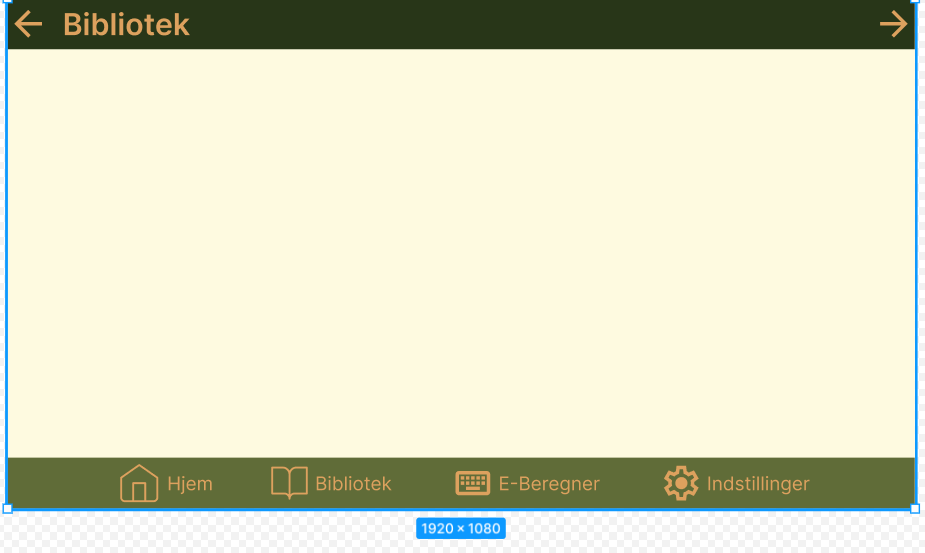
\includegraphics[width=\textwidth]{assets/Main_menu.png}}
    \caption{Viser Navigationsbjælkekonceptet}
\end{figure}

\section{Hovedmenuen}
\begin{figure}[H]
    \centering
    \fbox{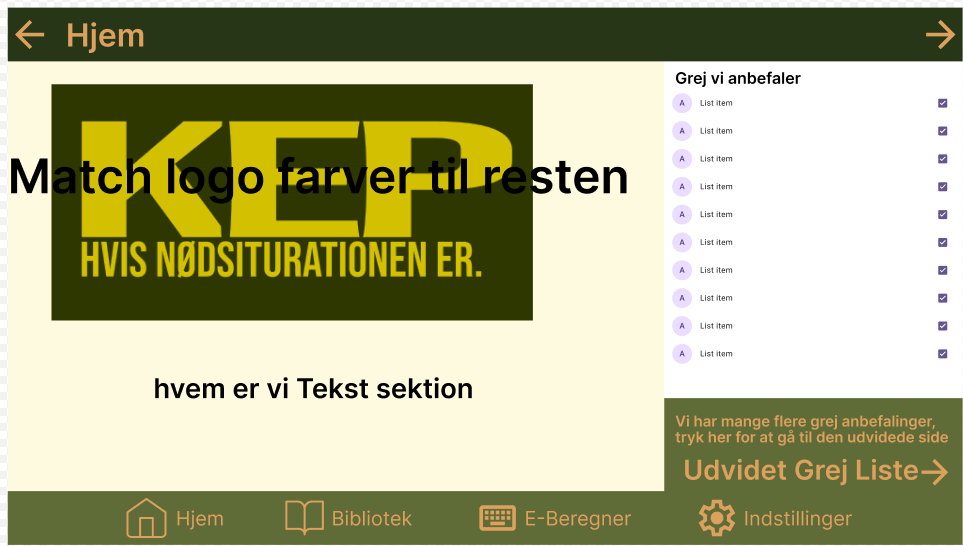
\includegraphics[width=\textwidth]{assets/Frontpage.png}}
    \caption{Viser frontpagekonceptet}
\end{figure}

\section{Manualbibliotekskoncept}
\begin{figure}[H]
    \centering
    \fbox{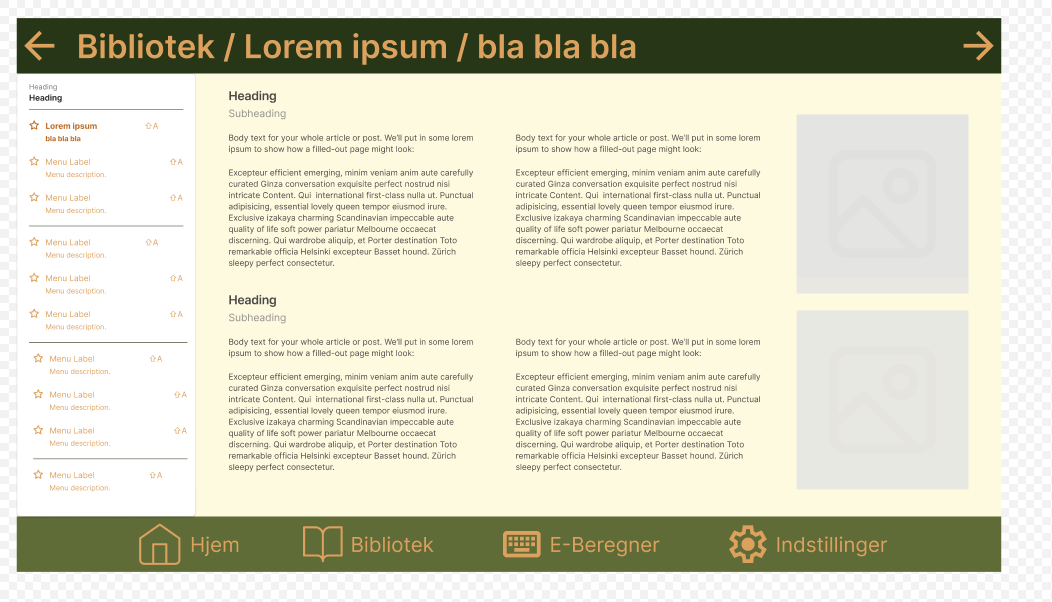
\includegraphics[width=\textwidth]{assets/library.png}}
    \caption{Viser manualbibliotekkonceptet}
\end{figure}

\section{Grejlistekoncept}
\begin{figure}[H]
    \centering
    \fbox{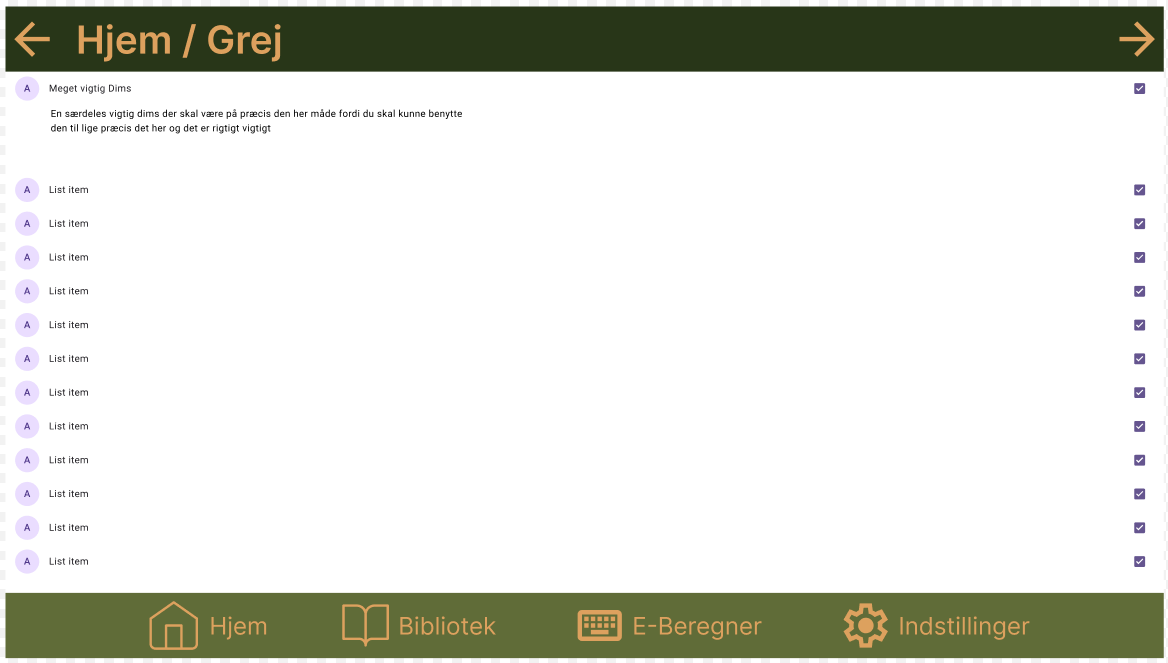
\includegraphics[width=\textwidth]{assets/Check_list.png  }}
    \caption{Viser grejlistekonceptet}
\end{figure}

\section{Ernæringsberegnerkoncept}
\begin{figure}[H]
    \centering
    \fbox{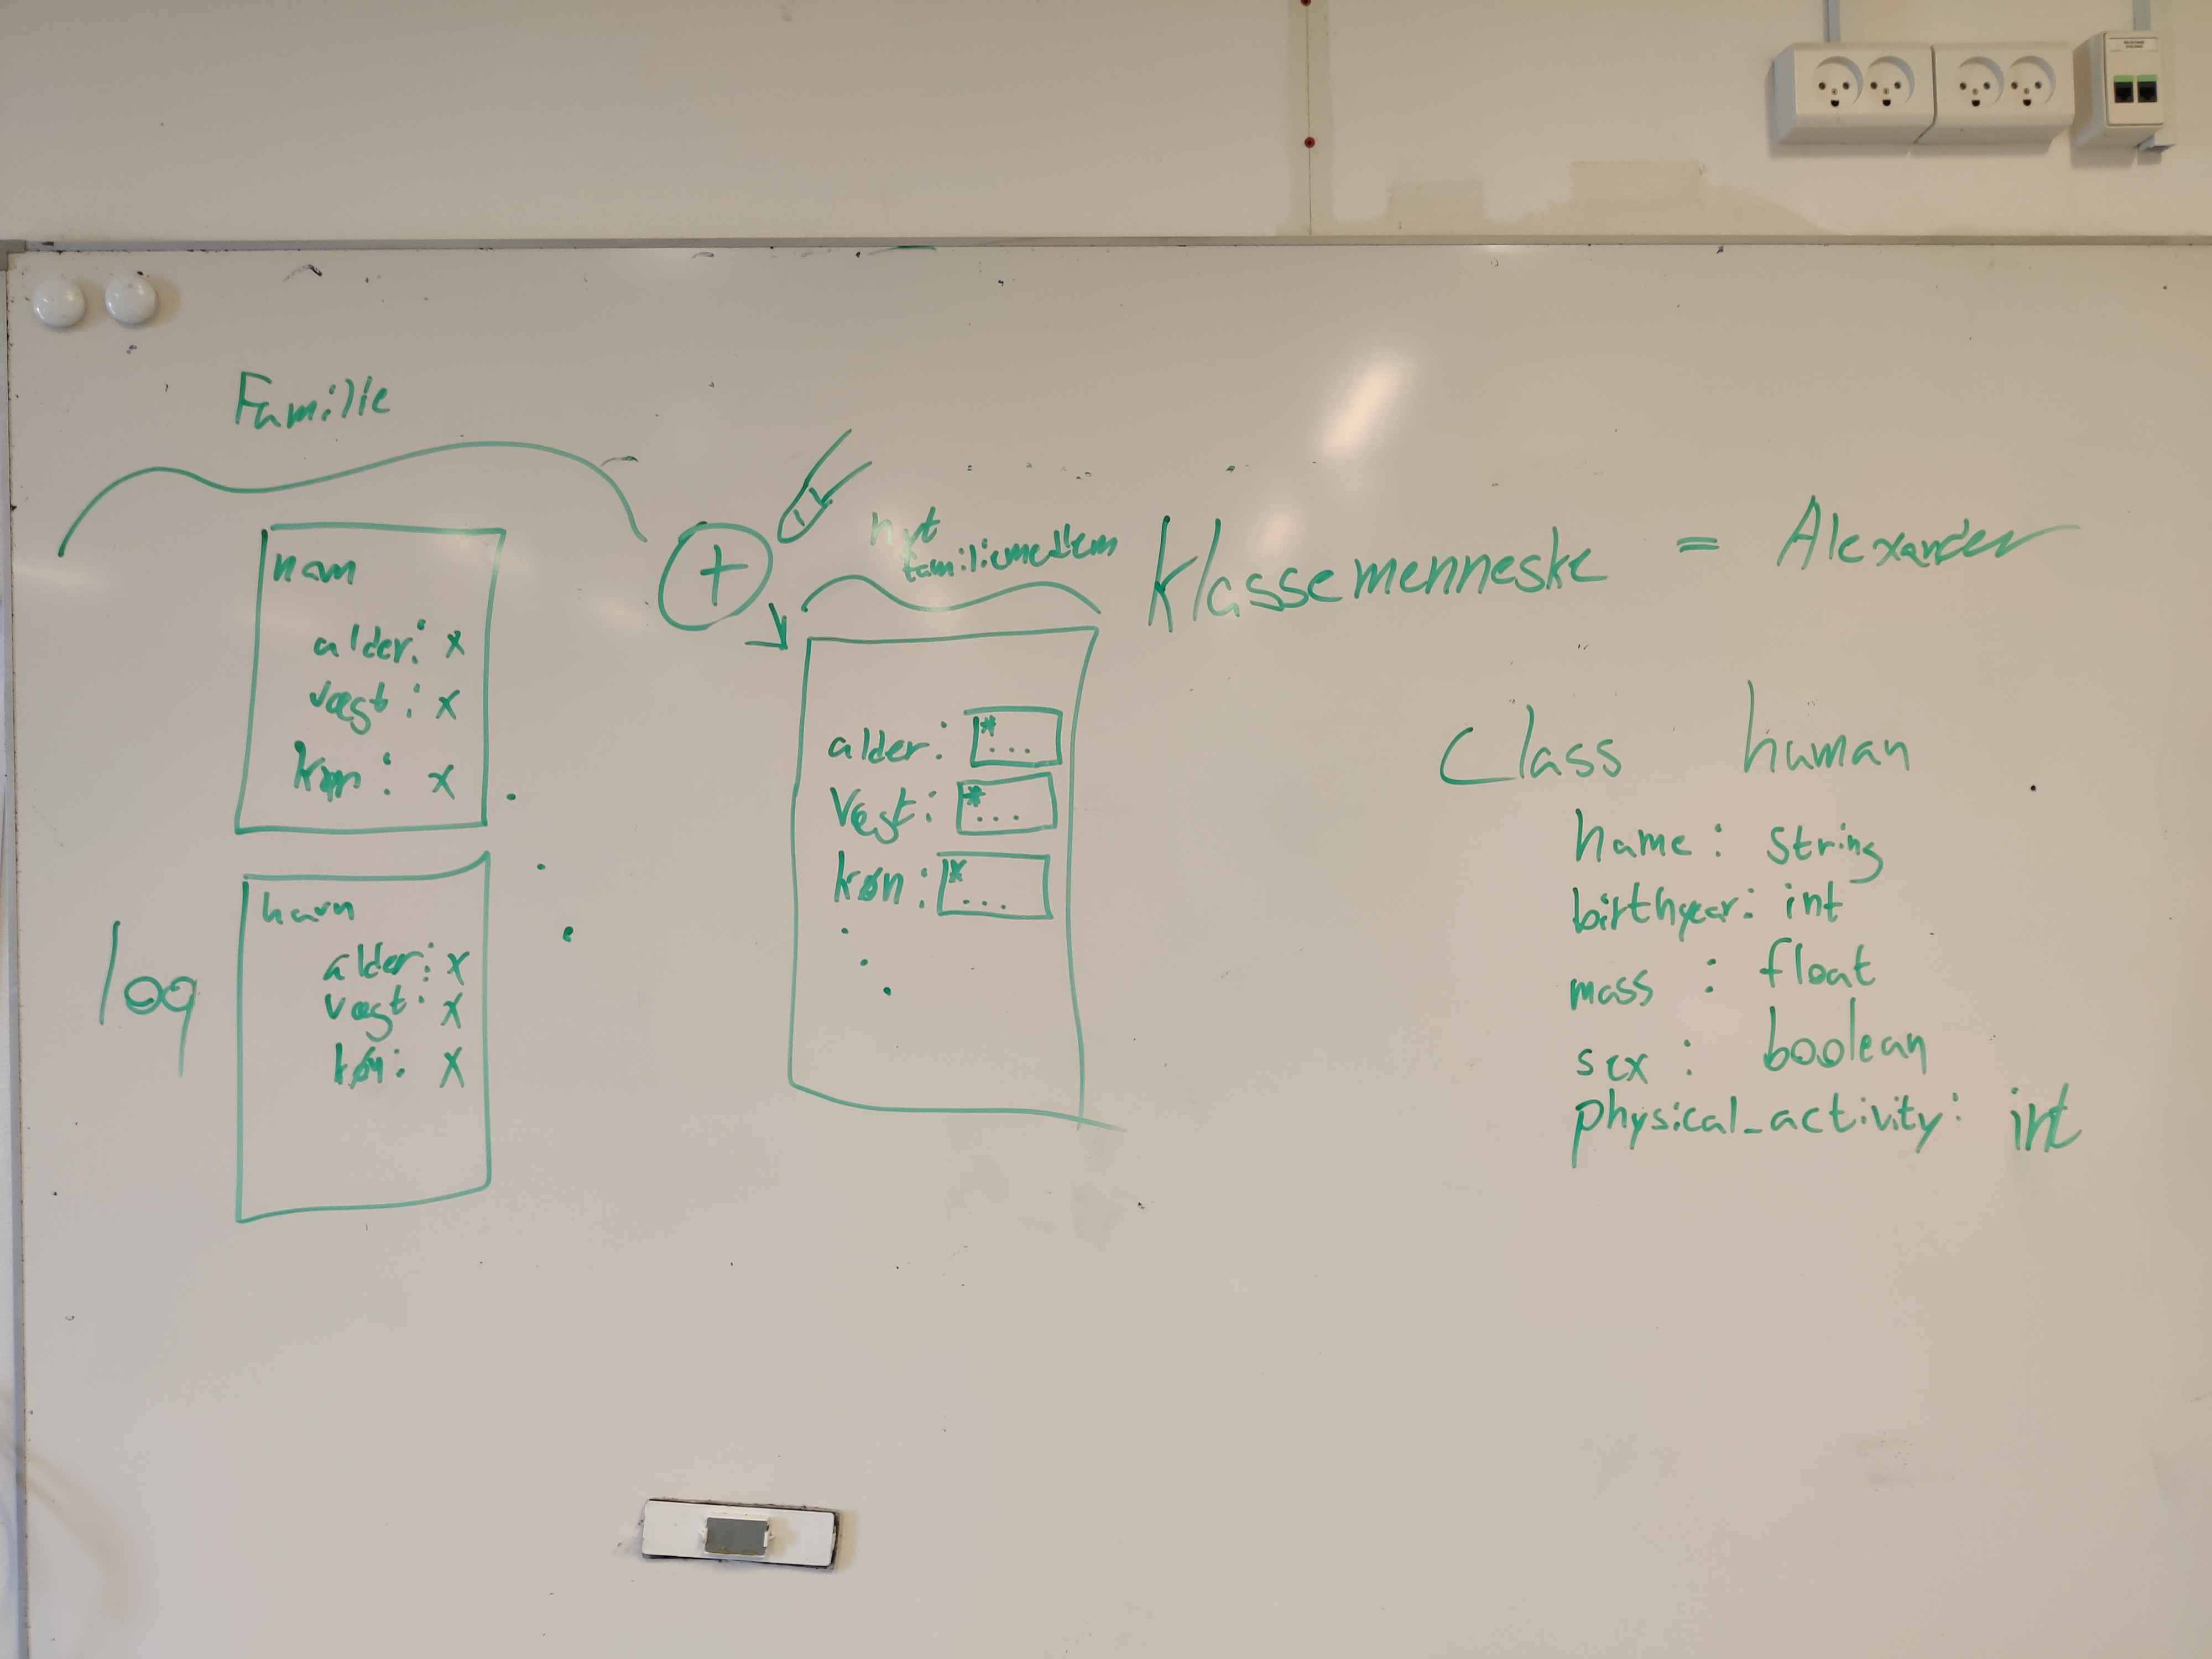
\includegraphics[width=\textwidth]{assets/Calculator_menu.png}}
    \caption{Viser ernæringsberegnerkonceptet}
\end{figure}

\section{Tilgængelighedsmenukoncept}
\begin{figure}[H]
    \centering
    \fbox{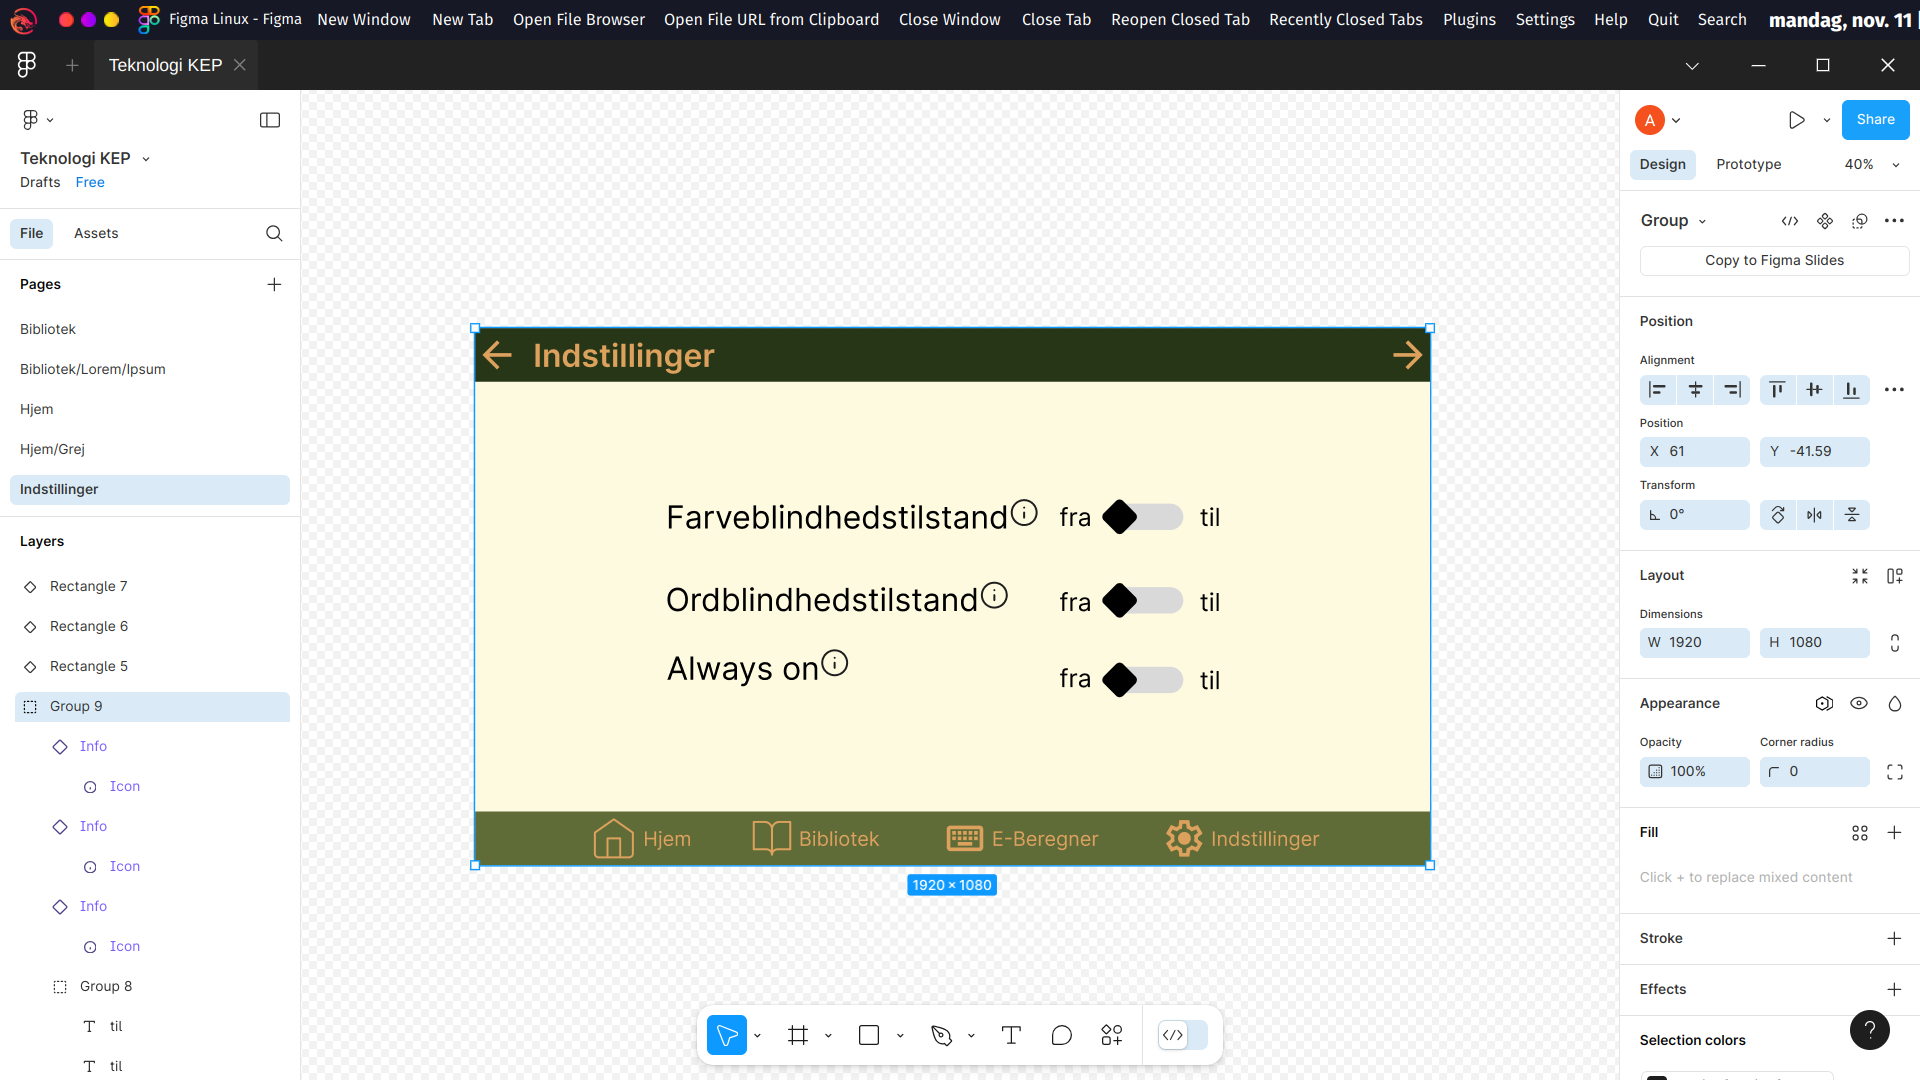
\includegraphics[width=\textwidth]{assets/Accessibility.png}}
    \caption{Viser tilgængelighedsmenukonceptet}
\end{figure}
\end{document}
